%!TEX ROOT=../../Diplomka.tex

\chapter{Teoretická část}

\section{Epilepsie}
Epilepsie je název pro soubor mozkových onemocnění charakterizovaných převážně recidivujícími a nepředvídatelnými výpadky normální mozkové aktivity, takzvanými epileptickými záchvaty. Epilepsie souhrnně označuje celou řadu mozkových dysfunkcí, které mohou mít různé příčiny na základě vrozených nebo získaných poruch.
\cite{1}

Podle definice zavedené International League Against Epilepsy (ILAE) a~International Bureau for Epilepsy (IBE) je epilepsie onemocněním mozku, které je charakteristické trvalou náchylností vytvářet epileptické záchvaty. Ty mají neurobiologické, kognitivní, psychologické a sociální důsledky. Epileptický záchvat je přechodný výskyt příznaků a/nebo symptomů, způsobených abnormálně vysokou nebo synchronní aktivitou neuronů v mozku, nebo nekontrolovanými elektrickými výboji v šedé kůře mozkové. Záchvaty přetrvávají několik sekund, minut, výjimečně hodin. Po odeznění záchvatu, v mezizáchvatovém období, může být nemocný zcela bez obtíží. \cite{2,1}

Epileptický záchvat je přechodný, s jasně viditelným nástupem a někdy méně zjevným koncem, což je způsobeno postiktálním stavem. Začátek a~konec epileptického záchvatu lze určit z chování jedince nebo EEG průběhů, nicméně tato dvě kritéria se nemusí vždy přesně shodovat. \cite{1}

Kognitivní dysfunkce se během záchvatu může projevovat jako problém s~vnímáním, pozorností, emocemi, pamětí, řečí nebo apraxií.

Abychom mohli diagnostikovat epilepsii u pacienta, je nutné, aby prožil alespoň jeden epileptický záchvat. Nestačí pouze rodová náchylnost k epilepsii nebo výskyt epileptiformních abnormalit v EEG. \cite{1}

Obecně se onemocnění objevuje ze dvou příčin. Může se jednat o již vrozenou vadu (primární epilepsie, způsobená nepříznivými vlivy během vývoje embrya), nebo o epilepsii získanou (sekundární, způsobenou pozdějším poškozením mozku úrazem, nádory apod.). Příčinou epileptických záchvatů může být jakákoliv léze mozku, která neurony částečně poškodí, ale úplně nezničí. Může se jednat i o dysfunkce v důsledku systémové poruchy, jako například hypoglykémie a hypoxie, nebo o důsledek úrazu mozku. \cite{2}

Základním patogenetickým mechanismem je epileptické ložisko (fokus, ohnisko). Jde o různě rozsáhlou populaci neuronů s patologickou elektrickou aktivitou. Patologie spočívá v porušení stavu klidové polarizace a v akční depolarizaci povrchové membrány neuronu, což způsobuje jeho hyperexcitabilitu. V ložisku dochází k abnormálním neuronálním výbojům s opakovanými salvami relativně vysokých a za sebou jdoucích potenciálů. Záchvaty mohou být ohraničené, nešíří se do okolí a klinická symptomatika je dána jejich lokalizací. V jiných případech se mohou šířit do celého mozku. \cite{2}

Přibližně 60 \% pacientů s epilepsií (0,4 \% populace) trpí nemocí kvůli epileptickému ložisku a 4,5 \% farmakorezistivních epileptiků by mohlo profitovat z operativního odstranění tohoto ložiska. Jak reportují různá epileptologická centra, za předpokladu, že dokáží přesně definovat a provést resekci epileptického ohniska, 30 – 85 \% (průměrně 60 \%) pacientů zůstává po zákroku bez záchvatů. \cite{6,4}

Důležitou roli v diagnostice epilepsie hraje EEG, v mezizáchvatovém období má význam především nález specifických grafoelementů, mezi které počítáme hroty, ostré vlny a komplexy hrot-vlna. Negativní nález v EEG však epilepsii nevylučuje. Moderní metodou je dlouhodobé video-EEG monitorování, kde současně zaznamenáváme EEG a klinické projevy. Pro zjištění strukturální léze a příčiny epilepsie jsou nejdůležitější CT a MRI, při podezření na arteriovenózní malformaci i angiografie. \cite{2}

V současnosti se typy záchvatů dělí dle oblasti mozku, která je abnormní aktivitou postižena. Toto dělení však není konečné \cite{71}:

\begin{itemize}
\item \textbf{Jednoduché parciální záchvaty } – postihují malé ložisko mozku, mohou se projevovat například poruchami smyslů, záleží na postižené oblasti mozku. Pacient zůstává při vědomí.
\item \textbf{Komplexní parciální záchvaty } – postihují rozsáhlou oblast mozku, způsobují automatický pohyb, narušují vědomí.
\item \textbf{Generalizované záchvaty bez křečí} – postihují celý mozek, jsou spojeny s krátkými výpadky vědomí, zahleděním se.
\item \textbf{Generalizované záchvaty s křečemi} – několikaminutové výpadky vědomí spojené typicky s pádem pacienta a tonickou křečí.
\end{itemize}

\subsection{Terapie}
Léčba epilepsie spojuje pravidelné dlouhodobé podávání antiepileptik s dodržování příslušné životosprávy (je třeba dodržovat pravidelný rytmus spánku a~bdění, nespat během dne, nepřijímat jednorázově velké množství tekutin, nepít alkohol a držet katogenní dietu). Podávání antiepileptik musí být pravidelné, lék nesmí být náhle vysazen a jeho dávkování je vždy řízeno odborníkem. \cite{2}

Pro těžké refrakterní epilepsie jsou dnes k dispozici antiepileptika tzv. III. generace. Některé dobře definované ložiskové epilepsie lze léčit i chirurgicky \cite{3}. Prognóza správně léčené epilepsie je celkem příznivá, záchvaty se většinou daří kompenzovat a zejména u dětí lze docílit i úplného vyléčení. \cite{2}

\subsection{Epileptologické zóny}
V současné době se již na epilepsii nahlíží jako na onemocnění zasahující spíše komplexní neurální sítě, nežli na jednotlivé ohraničené oblasti, tzv. zóny. Diagnostické metody definují zóny a léze na kortexu. Úspěšnost chirurgické léčby závisí na odstranění kritických částí epileptické sítě, zejména pak epileptogenní zóny, ve které dochází primárně k rozvoji záchvatů. Jednotlivé zóny jsou dnes dobře popsány a budu se jim věnovat v dalších podkapitolách. \cite{4}

\begin{figure}[!h]
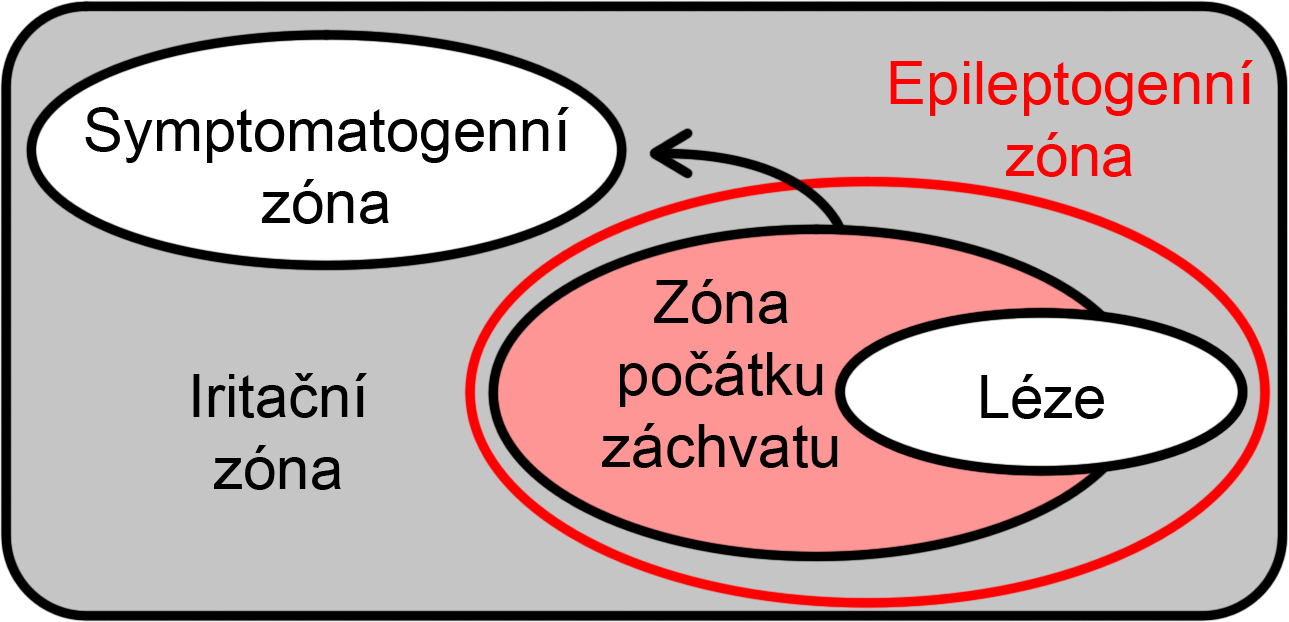
\includegraphics[scale = 0.2]{casti/teorie/zony.png}
\caption{Epileptologické zóny}
\end{figure}

\subsubsection{Symptomatogenní zóna}
Symptomatogenní zóna je část kortexu, která po aktivaci epileptoforním výbojem produkuje iktální symptomy. Tuto zónu je možné lokalizovat na základě iktální symptomatologie nebo pomocí analýzy video-EEG záznamu. Tato zóna se ve většině případů nepřekrývá s epileptogenní zónou, často však bývá s epileptogenní zónou propojena nebo se nachází v její těsné blízkosti. Nejpřesnější metodou určování pozice této zóny je přímá elektrická stimulace kortexu během invazivní explorace elektrodami. Tato procedura simuluje podobné podmínky jako při aktivaci epileptoformními výboji. \cite{4}

\subsubsection{Iritační zóna}
Tato zóna je definována jako část tkáně kortexu, generující typické mezizáchvatové výboje. Lokalizace této zóny se provádí pomocí EEG (skalpového nebo intrakraniálního), magnetoencefalografií nebo pomocí funkční magnetické rezonance (fMRI) spojené s EEG. Iritační zóna je často velmi rozsáhlá, může postihovat celou hemisféru. Její odstranění proto není nezbytně nutné, i když její zahrnutí do resekce zvyšuje šanci na dobrý pooperační výsledek. \cite{4}

\subsubsection{Zóna počátku záchvatu}
Zóna počátku záchvatu je klíčová část kortexu, ze které jsou spouštěny záchvaty a tvoří klíčovou část tzv. epileptogenní zóny. Nejčastěji lze určit její pozici z intrakraniálního EEG (vyjímečně ze skalpového EEG, lépe z~high density EEG), nebo pomocí SPECT (single photon emission computed tomografy). Skalpové EEG nám dokáže odhalit pouze přibližnou lokaci této zóny kvůli velkým plochám elektrod, jejich relativně malé citlivosti a kvůli relativně velké vzdálenosti od kortexu. Invazivní EEG je naopak velmi citlivé a zónu přesně určí pouze za předpokladu, že se elektroda nachází přímo uvnitř nebo nad touto oblastí. \cite{4}

\subsubsection{Epileptogenní strukturální léze}
Jde o abnormální mozkovou strukturu, která přímo způsobuje epilepsii. Nejčastěji je odhalena pomocí magnetické rezonance s vysokým rozlišením. Ne všechny léze na pacientově mozku jsou ovšem epileptogenní a nemusí s~epilepsií souviset. U nalezených lézí je nutné pomocí EEG ověřit, zda se jedná o~lézi zodpovědnou za pacientovy záchvaty. Dříve se mělo za to, že pouze úplná resekce takové léze vede k uzdravení pacienta. Objevily se však nové případy, ve kterých pomohla i pouze částečná resekce léze, čímž došlo k porušení klíčové struktury epileptické sítě. Na druhou stranu existují i případy, kdy ani celková resekce léze nepomohla. \cite{4}

\subsubsection{Zóna funkčního deficitu}
Zóna funkčního deficitu je část kortexu s abnormální funkčností v mezizáchvatovém období. Existuje více metod, jak určit funkčnost mozkové tkáně, a~to například pomocí psychologických a neurologických vyšetření, EEG, fMRI nebo SPECT. \cite{4}

\subsubsection{Epileptogenní zóna}
Epileptogenní zóna je pouze teoretickým konceptem, protože nelze určit její přesnou hranici. Je však zodpovědná za generování epileptických záchvatů. Pokud je pacient po operaci bez záchvatů, říkáme, že resekovaná oblast obsahovala epileptogenní zónu. \cite{4}

\subsubsection{Elokventní zóna}
Elokventní zóna je část kortexu, která brání úplné resekci epileptogenní zóny, protože plní nějakou významnou funkci jako je zrak nebo řeč. Poškození této zóny by vedlo k výraznému snížení kvality života pacienta. Zóna je lokalizována pomocí evokovaných potenciálů, MEG, fMRI nebo PET. \cite{4}




\section{Elektrofyziologická aktivita mozku}
Lidský mozek je nejkomplexnější organizovaná struktura, skládající se z cca 10\textsuperscript{10} neuronů v nejsvrchnější části v cerebrálním kortexu. Tyto buňky jsou aktivní jednotky obrovské signálové sítě, která zahrnuje 10\textsuperscript{14} propojení neboli synapsí. Během zpracovávání informací, tečou mozkem malé proudy, které můžeme měřit, tak je tomu v případě elektroencefalogramu (EEG). Můžeme také využít magnetické pole, které proudy vyvolávají (řádově fT), měřitelného pomocí magnetoencefalogramu (MEG). \cite{5}

\subsection{Magnetoencefalografie}
Počátky magnetoencefalografie se datují do šedesátých let dvacátého století, kdy se Cohen pokoušel měřit magnetické pole srdce a mozku pomocí měděných folií navinutých na feromagnetické jádro \cite{7}. Průlom přišel s vynálezem magnetometrů SQUID (superconducting quantum interference device), využívajících kvantový fenomén, nastávající při velmi nízkých teplotách, takzvaný Josephsonův jev. \cite{8}

Magnetoencefalograf je schopen zaznamenávat velmi slabá magnetická pole v řádech 10\textsuperscript{-15} Tesla (o několik řádů slabší než magnetický šum prostředí), která korelují s aktivitou neuronů v mozku. Jelikož je magnetické pole mozku tak slabé, jeho záznam je možný pouze v magneticky odstíněných místnostech \cite{6}. Fyzikální principy, na kterých MEG staví, jsou popsány v knize \cite{9}. 

Moderní MEG skenery s několika stovkami senzorů poskytují jemné prostorové rozlišení neuromagnetické aktivity mozku, díky čemuž je možné tvořit hypotézy o místech vzniku této aktivity \cite{6}. Na magnetoencefalografická data je také možné aplikovat algoritmy inverzních úloh. Proces je vcelku stejný, liší se pouze model přímé úlohy. 

MEG není předmětem této práce, nicméně jej uvádím pro úplnost.

\subsection{Elektroencefalografie}
EEG signál je záznamem potenciálů, vyvolaných proudy, které protékají během synaptické excitace dendrity neuronů cerebrálního kortexu a je následně promítán skrze pacientovu lebku až k elektrodám zaznamenávacího zařízení. EEG je typicky měřeno v řádech 10\textsuperscript{-6} voltů. Proudy v mozku jsou generovány převážně přechodem pozitivně nabitých iontů sodíku, draslíku a~vápníku a~negativně nabitých iontů chloru membránami neuronů \cite{10}. Elektrická aktivita mozku se dělí do dvou tříd: akční potenciály (AP) a postsynaptické potenciály (PSP). PSP se objeví při vyplavení neurotransmiteru presynaptickým neuronem. Dojde ke změně koncentračního gradientu, a tím ke změně membránového potenciálu. Velikost potenciálu jednoho izolovaného PSP je přímo úměrná počtu receptorů, které navázaly mediátor. Amplituda měřeného PSP klesá se vzdáleností od elektrod zaznamenávajícího přístroje. AP vzniká, jestliže membránový potenciál neuronu přesáhne jeho vnitřní prahovou hodnotu. AP se rychle šíří membránou neuronu, jeho amplituda neklesá díky napěťově citlivým sodíkovým a draslíkovým kanálkům. \cite{12}

Lidská lebka je tvořena mnoha různými vrstvami, jako jsou například skalp nebo lebka. Lebka signály generované mozkem tlumí asi stokrát víc, než ostatní měkké tkáně, proto jsme schopni zaznamenávat pouze signály větší populace aktivních neuronů. \cite{10}

Mozek také generuje signály o různých frekvencích. Jednotlivá pásma jsou označena jako delta (frekvence nižší než 4 Hz), théta (4-8 Hz), alfa (8-13 Hz), beta (13-30 Hz) a gama (30-45 Hz). \cite{10,11} Jednotlivá označení pásem jsou historická, dělená dle dominantní frekvence viditelné v EEG záznamu a~nereprezentují skutečné frekvenční spektrum EEG záznamů.  

Během epileptického záchvatu se v EEG signálu objeví výrazné změny, způsobené synchronní aktivitou neuronů. Jednou z charakteristik iktálního EEG je přítomnost hrotů a ostrých vln. Detekování záchvatů v EEG je potřebné nejen pro diagnózu, ale i pro terapii. \cite{14}

MEG a EEG je měření stejné mozkové aktivity, rozdílná je pouze pozorovaná veličina, kterou vyvolávají mozkem tekoucí proudy. Některé metody zpracování je tedy možné využít pro MEG i EEG, datový soubor je poté označován jako M/EEG nebo jen MEEG.

\subsubsection{Zpracování EEG signálu}
Časové a prostorové rozlišení (vysoká vzorkovací frekvence, velké množství elektrod) se obecně považuje za dobrou vlastnost, přináší to s sebou ovšem komplikaci v podobě množství dat, která jsou během měření signálu nasbírána. Nutností jsou tedy metody, umožňující detekovat události relevantní pro zpracování inverzní úlohy. Snažíme se z dat vyextrahovat takzvané ERP (event related potencials), EEG signál v časovém okně okolo nastalé události, na kterou chceme aplikovat inverzní úlohu. Události se mohou v datech objevovat náhodně (jako komplexy hrot-vlna u epileptiků), nebo periodicky (typicky u evokovaných potenciálů). Získané ERP jsou následně průměrovány, čímž je odstraněna náhodná aktivita, vyskytující se v jednotlivých ERP. Inverzní úloha je poté aplikována na zprůměrovaný signál.

\subsubsection{Artefakty}
EEG záznam je typicky zatížen šumy různých původů, takzvanými artefakty. Artefakty jsou nechtěné části signálu, které jsou způsobeny jinými zdroji, ne mozkem, a proto je nutné je v každém signálu identifikovat. Artefakty jsou nejčastěji způsobeny těmito zdroji:

\begin{itemize}
\item \textbf{Oční artefakty} – jsou způsobeny okohybnými svaly při pohybu očí nebo mrkání.
\item \textbf{Svalové artefakty} – interference s EMG, tyto signály zabírají širokou část frekvenčního pásma, může se jednat o rychlé hroty nebo delší oscilace.
\item \textbf{Artefakty srdeční aktivity} – interference s EKG, artefakty způsobené depolarizací srdce.
\item \textbf{Interference s rozvodnou sítí} – jedná se o naindukovaný signál rozvodné sítě o frekvenci 50 Hz nebo 60 Hz (a jejich vyšší harmonické) podle místního standardu.
\item \textbf{Pohyb elektrod} – pacientovým pohybem může dojít ke změně polohy elektrod a tím ke změně půlčlánkového potenciálu mezi skalpem a~elektrodou.
\item \textbf{Ostatní artefakty} – mohou se objevovat artefakty spojené se změnou půlčlánkového potenciálu, způsobené pocením pacienta nebo vysycháním vodivého gelu. Existují také elektrostatické artefakty, artefakty způsobené pohybem jazyka a mnoho dalších.
\end{itemize}

Jakmile identifikujeme části dat, obsahujících artefakty, můžeme buď taková data z dalšího zkoumání vyřadit, nebo některé typy artefaktů lze potlačit pomocí odpovídajících metod. \cite{13}

Nejčastější metody pro detekci artefaktů jsou založeny na lineární regresi a~snaží se eliminovat nejčastější artefakty, způsobené očními pohyby a mrkáním pomocí měření elektrookulogramu (EOG). \cite{15}

Komplexnější metody mohou být založeny na lineární dekompozici vícekanálového EEG. Takové metody předpokládají, že zdroj artefaktů a zdroj EEG jsou nezávislé a snaží se získat původní průběhy, pouze z EEG záznamu. \cite{15}

Artefakty je také možné klasifikovat pomocí klasifikátorů, tedy na základě příznaků, kterými je možné signál popsat. Příznaky je možné rozdělit do těchto kategorií:

\begin{itemize}
\item Statistické charakteristiky jako „špičatost“ (šikmost), entropie, trend a~extrémy. Špičatost lze použít pro detekci hrotů, charakteristických pro některé typy artefaktů (EOG, EKG), artefakt je indikován i vysokou hodnotou entropie během krátkého časového intervalu. \cite{16}
\item Pomocné měřené signály, pokud jsou k dispozici. Artefakt může být indikován pomocí vysoké hodnoty korelace EEG s EOG nebo EKG. \cite{17}
\item Frekvenční charakteristiky – zdroje signálu jsou často charakteristické svou energií v různých frekvenčních pásmech. \cite{17}
\item Amplituda signálu, promítnutého na skalpu, může indikovat jeho původ. \cite{18}
\end{itemize}

\subsubsection{Volba umístění a počtu elektrod}
Jednou ze zásadních otázek je, kolik elektrod je potřeba pro přesné určení zdroje aktivity. Teoreticky, čím víc elektrod, tím lepší prostorové rozlišení a~tedy přesnější výsledek. Některé články však ukázaly, že optimální rozdělení elektrod je s dvou- až třícentimetrovými rozestupy tak, aby rovnoměrně pokrývaly povrch hlavy. \cite{29,32,31}

Výsledky simulací ukazují, že vliv počtu elektrod na přesnost lokalizace zdroje signálu není lineární, přesnost roste od 25 do cca 100 elektrod (to závisí na zvolené metodě inverzní úlohy), poté přechází v plateau fázi. Simulace byla provedena naměřením EEG na 14 epileptických pacientech, EEG záznamy byly následně redukovány na nižší počty elektrod, tak aby rozestupy zůstaly uniformní.\cite{33}

\begin{figure}[!h]
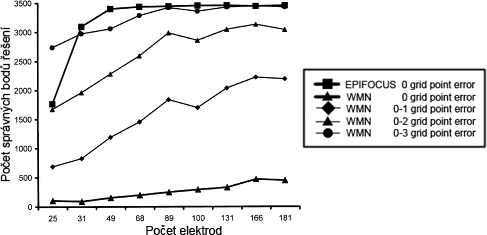
\includegraphics[scale=0.6]{casti/teorie/chybyInverze.png}
\caption{Přesnost výsledku inverzní úlohy v závislosti na počtu kanálů EEG záznamu \cite{72}}
\end{figure}

Pro algoritmus EPIFOCUS bylo dosaženo maximální přesnosti už při 68 elektrodách. Algoritmus WMN (weighted minimum norm) dosahoval nižší přesnosti lokalizace, proto byly zahrnuty i počty správných řešení pro různé rozsahy tolerancí, maximální přesnosti bylo však vždy dosaženo pro 166 elektrod. \cite{33}

Některé články navrhovaly, že pro zlepšení prostorového rozlišení v místě, kde se předpokládá přítomnost zdroje signálů, by se měla zvýšit koncentrace elektrod \cite{34}. To mělo hlavně vyřešit problém s nízkým počtem elektrod systémů 10-20. Novější články argumentují tím, že dnes již jsou systémy s dostatečně velkým počtem elektrod levné a dostupné a některé dokonce vyvracejí navržený nápad vlastními výzkumy.

\begin{figure}[!h]
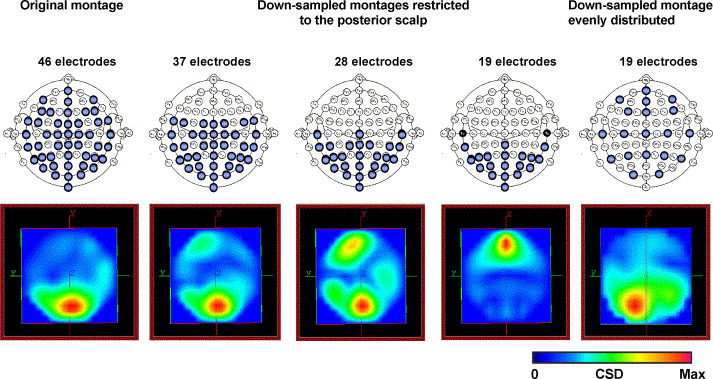
\includegraphics[width=1.0\textwidth]{casti/teorie/rozlozeniElektrod.jpg}
\caption{Vliv nerovnoměrného rozmístění elektrod na pacientově skalpu \cite{73}}
\end{figure}

Při zkoumání efektu rozdělení elektrod na lokalizaci zdroje bylo využito algoritmu Loreta v 3-shell sphere modelu hlavy (viz \ref{3-shell-sphere}). Inverzní úloha byla aplikována na vizuální evokované potenciály, aktivita je tedy očekávána v~okcipitální oblasti mozku. Lokalizace byla nejprve provedena na systému se 46 rovnoměrně rozmístěnými elektrodami (vlevo). V dalších pokusech byly vyřazovány elektrody z frontální oblasti. V posledním případě (vpravo) je zobrazen set s 19 rovnoměrně rozmístěnými elektrodami a aktivita se opět objevuje v předpokládané oblasti. Pro aplikaci inverzních úloh je tedy nutné zachovat rovnoměrné rozmístění elektrod. 


\subsubsection{Volba reference}
Nutnost volby reference je brána jako jedna z nevýhod EEG oproti MEG, aktivní reference může vést k problémům při interpretaci dat. \cite{36,37}

Pro výpočty inverzní úlohy pomocí SPM12 je nutné zaznamenat EEG signál pomocí referenčního zapojení. Jako reference může být použita některá z~elektrod (umístěná například na ušní boltec nebo kořen nosu), nebo je možné využít průměrné reference (referenční hodnota je vypočtena jako průměr hodnot všech elektrod). Dokumentace SPM12 dokonce doporučuje, aby byla data vždy pro jistotu přereferencována na průměrnou referenci, aby byly splněny předpoklady, ze kterých vychází výpočet inverzního problému. \cite{35} 

Podle \cite{38} je však volba reference u unipolárního zapojení irelevantní, protože různé reference nemění vztah mezi jednotlivými elektrodami. Mění pouze aditivní konstantu, která však nemá žádný fyzikální význam. Ekvipotenciální mapy se nijak nemění.

Bipolární záznam poskytuje měření lokálního zdroje, které je nevhodné pro účely inverzní úlohy, protože reprezentují měření skalpového proudu pouze ve směru bipolárního páru. \cite{31}


\subsubsection{Možné chyby měření}
Jednou z chyb, se kterou se můžeme setkat, je nepřesnost při snímání pozic elektrod digitizérem. Vliv nepřesné lokalizace elektrod byl testován v \cite{39}, kde byla simulována nepřesnost snímání elektrod náhodnými posuny v okruhu do 1 centimetru. Studie ukázala, že vliv této nepřesnosti na správnost výsledku inverzní úlohy je malý a oproti chybě, způsobené šumem v datech, zanedbatelný.

Další chybou, se kterou se můžeme v praxi setkat, je kanál kontaminovaný artefakty kvůli špatnému kontaktu se skalpem pacienta nebo kvůli chybě zesilovače. Takové elektrody je možné z inverzní úlohy jednoduše vyřadit, aniž by byla ovlivněna přesnost lokalizace aktivní oblasti mozku. \cite{29}





\section{Zdrojová analýza}
Během posledních několika dekád bylo vyvinuto velké množství technik vyhodnocování neinvazivního měření mozkové aktivity. Jednou z nich je zdrojová analýza, jejíž snahou je z elektroencefalografických (EEG) nebo magnetoencefalografických (MEG) dat (souhrnně označovaná jako M/EEG) lokalizovat zdroj pozorované aktivity. Na naměřená data jsou aplikovány techniky zpracování signálu s~cílem odhadnout proudové zdroje v mozku tak, aby bylo dosaženo nejlepší shody s naměřenými daty. Tento proces se nazývá inverzní úloha. \cite{20}

Metody zdrojové analýzy mohou být využity v epileptologii. Výsledky algoritmů jsou schopny správně lokalizovat epileptogenní zónu. Tato problematika je předmětem zkoumání mnoha článků, příkladem jsou \cite{59}, \cite{60}, \cite{62} nebo \cite{33}.

Prvním krokem zdrojové lokalizace je snaha nalézt skalpové potenciály, vyvolané hypotetickými proudovými dipóly, nebo obecněji distribucí proudů. Jinými slovy, definujeme, jaké EEG signály vyvolá aktivace daného místa v~mozku. Tento krok se nazývá přímá úloha (forward problem) a je nedílnou součástí výpočtu inverzní úlohy \cite{19}. Pomocí modelu, vzniklého při vypočtu přímé úlohy a naměřených EEG dat, se můžeme zpětně dopracovat ke zdrojům, které dobře modelují naměřenou aktivitu – inverzní úloha (inverse problem) \cite{20}. Přesnost, se kterou mohou být zdroje lokalizovány, je ovlivněna řadou faktorů jako například nepřesnostmi v modelu hlavy, nepřesnostmi v metodě inverzní úlohy nebo šumem v datech. \cite{20,23}


\subsection{Přímá úloha}
\label{primaUloha}
Cílem moderních metod pro zpracování EEG signálů je lokalizovat zdroj aktivity v anatomicky přesném modelu hlavy. Výsledky je poté možné porovnat s dalšími vizualizačními technikami. Na geometricky (anatomicky) a elektromagneticky přesném (přesná vodivost pro EEG nebo permeabilita v~případě MEG) modelu závisí také správnost výsledků inverzní úlohy. \cite{29} 

Dopředný model hlavy je v základu definován Maxwellovými rovnicemi, kterými je možné popsat proudové dipóly pomocí jejich orientace $\vec{j}$ a jejich pozice $\vec{r}$. Těmito parametry modelujeme EEG data $Y=f(\vec{j}, \vec{r})$. Funkce $f$ je také závislá na pozici senzorů, geometrii hlavy, vodivosti jednotlivých tkání hlavy a~může být vyjádřena analyticky nebo numericky \cite{25}. Při výpočtu modelu je vygenerována transformační matice (tzv. lead field matrix), která je násobena vektorem proudové hustoty. Výsledkem této multiplikace jsou EEG potenciály, vyvolané daným rozložením proudů. Ty jsou dále využity k porovnání s naměřenými daty a k odhadu zdrojů aktivity. Rozdíl mezi modelovanými a~skutečnými EEG potenciály slouží jako míra správnosti odhadu zdrojů. \cite{29}

Existuje několik možností, jak vytvořit model hlavy. Modely se mohou lišit svou komplexností, výpočetní náročností, liší se i modely pro EEG a MEG data. Pro EEG data máme v SPM12 toolboxu možnost volby mezi dvěma modely. Prvním z nich je takzvaný 3-shell sphere model. Jde o modelování hlavy pomocí soustředných koulí. Jednotlivé koule oddělují vodivostní pásma, která jsou v~modelu uvažována. Tento model je nejjednodušší, a proto jsou výpočty s ním nejrychlejší. Nesprávně však modeluje hlavu jako sféru a~vodivosti jednotlivých koulí považuje za homogenní. Pro nevýhody prvního modelu je častěji využíván BEM (Boundary element model). Ten modeluje jednotlivé objemy tkání hlavy (hmota mozková, lebka, skalp), jejichž tvary jsou odvozeny ze snímků MRI nebo CT. Takový model je realistický, ale pomalý na výpočet. Může být zatížen chybami, pokud je počítán ze MRI snímků s~malým rozlišením. BEM modeluje tři hlavní změny ve vodivosti hlavy, hranice pokožky hlavy a vzduchu, hranice pokožky hlavy a lebky, hranici lebky a~mozku samotného. Čtvrtá vodivostní změna, mezi bílou a šedou hmotou, je důležitá pouze pro některé algoritmy \cite{24} a SPM12 ji nemodeluje. Další možností modelu hlavy, která však není v SPM12 toolboxu dostupná, je FEM (finite element model), modelování pomocí metody konečných prvků. Takový model hlavy umožňuje definovat vodivosti jednotlivých voxelů a umožňuje tak definovat porušení celistvostí jednotlivých tkání hlavy a mozku. Takto detailní anatomické informace ale nejsou většinou dostupné, a proto se FEM používá jen zřídka. \cite{29}

\begin{figure}[!h]
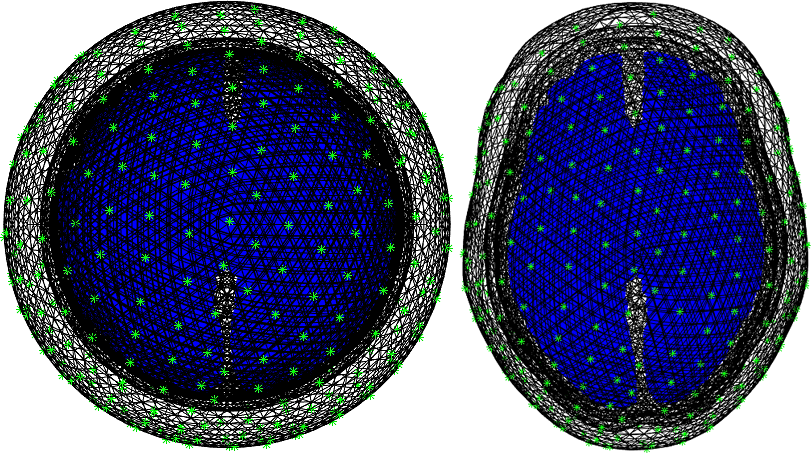
\includegraphics[width=1.0\textwidth]{casti/teorie/modely.png}
\caption{3-Shell Sphere a BEM modely hlavy}
\label{3-shell-sphere}
\end{figure}

Zjištění přesného rozložení jednotlivých hranic tkání mozku z MRI snímku je složitým problémem kvůli nízkým rozdílům kontrastů různých tkání. Záleží také na vážení MRI snímku (T1, T2 nebo protondensitní) \cite{24}. SPM12 využívá Forwinv toolboxu, který tento problém řeší s využitím standardního MNI mozku, který je geometricky transformován tak, aby výsledný model mozku vypadal jako ten z MRI snímků. Tento krok se nazývá prostorová normalizace (spatial normalization). Standardní MNI (Montreal Neurological Institute) mozek je vzorový model mozku, reprezentující normální populaci. Je průměrem 305 MRI snímků hlav zdravých lidí \cite{69}. Model hlavy, odvozený čistě z MRI nebo CT snímků, nikdy nebude stoprocentně shodný s modelem vypočteným pomocí prostorové normalizace. Odlišnost modelů však není natolik výrazná, aby byly výsledky inverzní úlohy jakkoli ovlivněny \cite{24}.

Vodivosti jednotlivých tkání jsou převzaté z literatury, z článků \cite{26} \cite{27} a~\cite{21}. Tkáně jsou považovány za čistě odporové, kapacitní a indukční efekty jsou zanedbány. Impedance tkání jsou tedy považovány za frekvenčně nezávislé. \cite{22} 

Přímá úloha také vymezuje oblasti, ve kterých se mohou zdroje aktivity nacházet. Zamezuje tak řešením, kdy by se zdroj aktivity mohl objevit mimo hlavu (takové řešení by teoreticky mohlo lépe odpovídat naměřeným datům, než jiná řešení). \cite{29}

\subsubsection{Měření pozic elektrod}
Digitalizace pozic senzorů se provádí takzvaným digitizérem. Jedná se o~systém, skládající se z ukazovátka a kamerového systému. Ukazovátko je vybavené orientačními body. Jeho špička se umístí na pozici měřené elektrody a~kamerový systém zaznamená pozice orientačních bodů. Ze znalosti pozic orientačních bodů a rozměrů ukazovátka je vypočtena pozice měřené elektrody v~prostoru.

Aby bylo zamezeno chybám, spojeným s případy, kdy se pacient během měření pohne a znehodnotí tak dosavadní měření, další orientační body jsou umístěny přímo na pacientově hlavě. Můžeme tak vždy zjistit polohu elektrody ve vztahu k aktuálnímu natočení a pozici pacientovy hlavy.

Během tohoto procesu je možné také nasnímat body, popisující tvar hlavy (headshape body), body na pacientově skalpu a obličeji. Tyto body jsou využívány pro zlepšení tvaru modelu pacientova mozku nebo pro zpřesnění koregistrace.

\subsubsection{Koregistrace}
Abychom byli schopni definovat řešení inverzní úlohy v MRI snímku pacientova mozku, potřebujeme znát pozice elektrod na pacientově skalpu, musíme provést sjednocení souřadnicových systémů MRI snímku a prostoru elektrod. Tento krok se nazývá koregistrace.
 
Souřadnicové systémy jsou sjednoceny výpočtem translačních a rotačních transformací prostorů. Parametry transformací jsou obvykle získány díky změření pozic tří orientačních bodů na pacientově lebce, jejichž polohu známe také v prostoru MRI snímku. Body jsou označovány jako fiducials. Nejčastěji používané fiducials jsou nasion a levý a pravý pre aurikulární bod, tedy kořen nosu a bod na levém a pravém uchu. \cite{29}

I když jsou pre-aurikulární body používané nejčastěji, je těžké tyto body lokalizovat přesně. Chyba v lokalizaci bodů vede k chybám v koregistraci (elektrody se mohou po transformaci nacházet například nad skalpem modelu), což ovlivňuje správnost inverzní úlohy. SPM12 toolbox řeší tento problém tak, že nejdříve napočítá transformaci z bodů fiducials a poté je koregistrace zpřesněna pomocí bodů, o kterých víme, že se nacházejí na skalpu pacienta. Mezi tyto body patří pozice elektrod, je ale možné využít headshape bodů. Počáteční transformace je zpřesněna metodou nejmenších čtverců. Nejlepší transformace minimalizuje sumu druhých mocnin vzdáleností bodů (pozic elektrod a headshape bodů) a skalpu.

Obecně je možné použít pro koregistraci jakékoliv tři body, známé v~obou souřadných systémech, je tedy možné využít například pozic některých elektrod, pokud známe jejich pozice v prostoru MRI. V takovém případě doporučuji volit body co nejvíce vzdálené od sebe, nepřesnost lokalizace vzdálených bodů vede k menší chybě koregistrace.

\begin{figure}[!h]
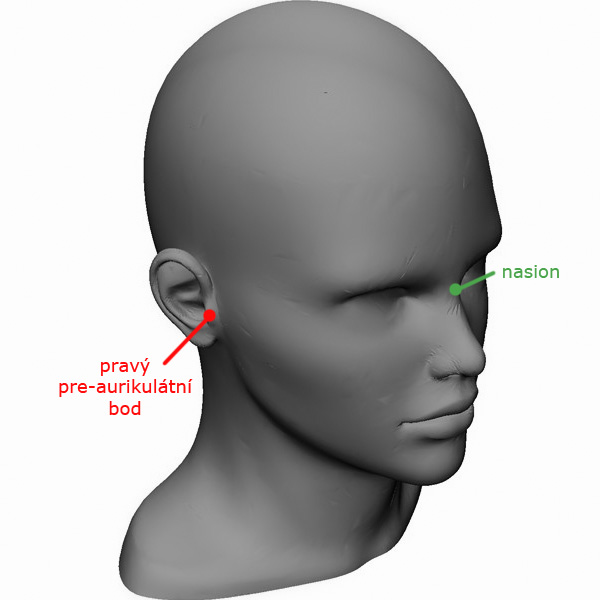
\includegraphics[scale=0.32]{casti/teorie/Fiducials.jpg}
\caption{Pozice bodů fiducials}
\end{figure}

\subsection{Inverzní úloha}
Lokalizace aktivní části mozku při dané mentální úloze je primárním záměrem zobrazovacích metod, zaměřených na centrální nervovou soustavu. Velká část výzkumu se zabývá zobrazováním pomocí PET (pozitronová emisní tomografie) a fMRI (funkční magnetická rezonance)\cite{30}. Tyto metody však nejsou ideální, pokud je otázkou, ve kterém časovém okamžiku během mentální úlohy byly jednotlivé části mozku aktivní. Pro řešení takového případu je nutné používat metody, které měří mozkovou aktivitu přímo, tedy elektroencefalografii nebo magnetoencefalografii. M/EEG signály nepřináší přímé důkazy o~umístění zdrojů aktivit. Jediný způsob, jak lokalizovat zdroje, je výpočtem inverzního problému. Inverzní úlohu lze vyřešit pouze pokud zavedeme předpoklady, které definují, jakým způsobem jsou M/EEG signály generovány. \cite{29} 

\subsubsection{Volba inverzní úlohy}
Obecně se algoritmy, řešící inverzní úlohu, snaží najít takové intrakraniální zdroje, které vytvářejí potenciály, shodné s potenciály naměřenými na skalpu pacienta. Základním problémem je však víceznačnost řešení. Naměřené skalpové potenciály lze obecně vysvětlit nekonečným množstvím konfigurací intrakraniálních zdrojů. Abychom byli schopni vyřešit takovou úlohu jednoznačně, je potřeba zavést předpoklady o zdrojích a vodivostech jednotlivých tkání. \cite{40,29}

\paragraph{Přeurčené modely}
Tyto metody inverze staví na dvou hypotézách: 

\begin{itemize}
\item Naměřený M/EEG signál se snaží vysvětlit pouze malým počtem proudových dipólů. 
\item Tyto dipóly jsou velmi fokální. 
\end{itemize}

Aby bylo dosaženo jednoznačného řešení, počet odhadovaných parametrů dipólů (každý dipól je popsán 6 parametry, 3 pro pozici, 2 pro natočení a 1 pro amplitudu) musí být nižší nebo roven počtu nezávislých měření (tedy počtu elektrod). Z procházeného stavového prostoru jsou postupně vybírány dipóly, pomocí nichž jsou vypočteny potenciálové mapy, které jsou následně porovnány s naměřenými potenciálovými mapami. Optimální řešení je zvoleno metodou nejmenších čtverců. Takové řešení minimalizuje součet čtverců rozdílů. Kvůli časové náročnosti výpočtů není možné projít stavový prostor celý, proto se přistupuje k optimalizačním procedurám, u kterých ale existuje risk uváznutí v lokálním optimu. Výpočetní nároky také rostou s~počtem hledaných dipólů, proto se typicky nepoužívá maximální možný počet dipólů daný měřením. \cite{28,29}

Přeurčené modely se snaží vytvořit model podle předpisu:
\begin{equation}
Y = L\vec{j} + e
\end{equation}

Kde $L=f(\vec{r})$ je transformační matice, $\vec{j}$ je orientace dipólů a $\vec{r}$ označuje polohu dipólů. Veličina $e$ označuje šum, který se objevuje v datech. Rovnice je řešena ve smyslu nejmenších čtverců. \cite{25}

Klíčovou otázkou zůstává, kolik aktivních zdrojů (tedy počet dipólů) se v~datech očekává. Tento parametr musí určit uživatel na základě svých zkušeností. Nejčastěji se počet volí na základě znalosti o tom, co data obsahují. Pro evokované potenciály nebo eliptické výboje se předpokládá velmi nízký počet aktivních zdrojů. Naopak aktivity, u kterých se očekává paralelní aktivace více míst, musí být popsány více dipóly. Existují také studie, navrhující metody, pro odhad početu dipólů na základě PET nebo fMRI. \cite{41,29}

Metoda lokalizace proudových dipólů je užitečná pro svou schopnost reprezentovat pozorovaná EEG data pomocí malého množství dobře interpretovatelných parametrů. Popsání mozkové aktivity pomocí malého počtu zdrojů zjednodušuje analýzu konektivity mezi těmito zdroji (dynamické kauzální modelování). \cite{42}

Nelze mezi sebou porovnávat modely s různými počty odhadovaných dipólů pouze na základě odchylky pozorovaných a modelovaných dat, protože s rostoucím počtem dipólů přesněji modelujeme pozorovanou aktivitu. Je však možné porovnávat takové modely na základě parametrů věrohodnosti (likelihood), které berou v potaz komplexnost modelů. \cite{42}

V SPM12 toolboxu je takováto metoda naimplementována pod zkratkou VB-ECDs (Variational Bayes Equivalent Current Dipoles) podle článku \cite{42}. Oproti jiným inverzním metodám ECD také umožňuje nadefinovat apriorní pravděpodobnost výskytu zdrojů aktivity, která může být vystavěna na empirických znalostech nebo dřívějších pozorováních pacienta. Tato pravděpodobnost může rozřešit situace, kdy různé dipóly modelují EEG data stejně dobře a model neposkytuje dostatek důkazů ve prospěch jednoho z řešení. \cite{28,42}

Existují přístupy optimalizace odhadu dipólů, takzvané „iterativní podmíněné režimy“ (ICM, iterative conditional mode). Je však známo, že tyto techniky nejsou invariantní a také nepočítají likelihood modelu \cite{42}. Tento optimalizační přístup je vhodný pro neinformované metody, kdy není definována apriorní pravděpodobnost, protože postup umožňuje projití lokálních maxim účelové funkce a nalezení dobrého výsledku. \cite{28}

\paragraph{Nedourčené modely}
Tyto metody jsou vhodné v případech, kdy počet dipólů není znám a nelze jej určit. Nedodurčené modely rekonstruují mozkovou aktivitu v každém bodě modelu pomocí tisíců dipólů fixní orientace rovnoměrně rozmístěných v modelu hlavy. Snahou je nalézt takovou unikátní konfiguraci zdrojových bodů, které co nejlépe odpovídají naměřeným datům. Problémem je to, že konfigurací zdrojových bodů, které přesně odpovídají naměřeným datům, je nekonečně velké množství. To znamená, že takový inverzní problém je nedostatečně podmíněný. Je tedy nutné přistoupit na další předpoklady, abychom byli schopni vybrat nejlepší řešení. V literatuře je navrženo mnoho různých omezení, která vedou k dobrým řešením. Některá jsou matematická, některá staví na znalostech fyziologie a některá vycházejí ze závěrů dalších zobrazovacích metod. Správnost těchto omezení je klíčová pro validitu řešení inverzního problému. \cite{29}

Nedourčený model je založený na lineárním mapování mezi dipólovými momenty fixního počtu dipólů a souborem signálů naměřených EEG nebo MEG. Tento vztah je dán vzorcem: 
\begin{equation}
Y = LJ + e
\end{equation}

Kde $Y$ je datový set M/EEG:
\begin{equation*}
Y \in {\rm I\!R}^{N_c \times N_n}
\end{equation*}

$N_c$ je počet senzorů a $N_n$ je počet časových vzorků, $J$ označuje neurální aktivitu zdrojů:
\begin{equation*}
J \in {\rm I\!R}^{N_d \times N_n}
\end{equation*}

$N_d$ je počet proudových dipólů distribuovaných modelem hlavy. Ty mají fixní orientaci kolmou k povrchu hlavy. Tyto dva sety jsou spojeny lead field matrix $L$:
\begin{equation*}
L \in {\rm I\!R}^{N_c \times N_d}
\end{equation*}

Měření je zatíženo Gaussovským šumem $e$ s nulovou střední hodnotou a~kovarianční maticí $Q_e$. Protože pro nedourčené modely obecně platí, že $N_d >> N_c$, pak nelze provést inverzi matice $L$ a tedy odhad $J$ nelze provést přímo. Za předpokladu, že $J$ má nulovou střední hodnotu a kovarianční matici $Q$, Bayesovská statistika umožňuje vytvořit odhad $\hat{J} = E[p(J|Y)]$, kde:
\begin{equation}
p(J|Y) = \frac{p(Y|J)p(J)}{p(Y)}
\end{equation}

Přičemž $p(Y)$ uvažovat nemusíme, protože je pro daná data konstantní a~vztah se nám zjednoduší:
\begin{equation}
p(J|Y) = p(Y|J)p(J)
\end{equation}

Jinými slovy se snažíme získat proudové rozložení $J$ založení na datovém souboru $Y$, kde $p(J)$ je stanovisko o zdrojích aktivity, které jsme stanovili ještě před měřením dat. Věrohodnost $p(Y|J)$ určuje pravděpodobnost, že dané proudové dipóly generují taková EEG data. $p(Y|J)$ má Gaussovské rozdělení $\mathcal{N}(LJ,Q_e)$. Protože $p(Y|J)$ i $p(J)$ mají normální rozdělení, můžeme psát:
\begin{equation}
p(Y|J)p(J) \propto \Theta = exp(-\frac{1}{2} (LJ-Y)^T Q^{-1}_e (LJ-Y)-\frac{1}{2}J^T Q^{-1} J)
\end{equation}

Optimální hodnoty aktivity zdrojů minimalizují $\Theta$, což odpovídá takové aktivitě, jejíž gradient $log(\Theta)$ je nulový:
\begin{equation}
\frac{d(log(\Theta))}{dJ} \Bigg\vert_{J = \hat{J}} = 0 = -L^T Q^{-1}_e (L\hat{J}-Y) - Q^{-1} \hat{J} 
\end{equation}

Z čehož je možné vyjádřit $\hat{J}$:
\begin{equation}
\hat{J} = Q L^T (Q_e + LQL^T)^{-1} Y
\label{vyslednaRovnice}
\end{equation}

Protože data $Y$ jsou známá a transformační matici $L$ lze vypočítat z modelu hlavy, potřebujeme pouze odhadnout kovarianční matice a jsme schopni získat zdrojové proudy $J$ v jediném algebraickém kroku.

Přesnost výpočtu velmi záleží na přesnosti, se kterou jsme schopni určit $Q$ a~$Q_e$. Předpokládáme, že kovarianční matice šumu senzorů má tvar:
\begin{equation*}
Q_e=h_0 I_{N_c}
\end{equation*}
Kde $I_{N_c}$ je jednotková matice o rozměru $N_c$ a $h_0$ je rozptyl šumu senzorů. \cite{74}

V následujících kapitolách si ukážeme několik příkladů omezení pro výběr řešení, nelze však pokrýt všechny algoritmy, protože jich je nesčetné množství. Nové algoritmy často vznikají jen drobnými úpravami již existujících algoritmů.





\paragraph{Minimum norm - MN}
\label{minimumNorm}
Minimum norm je obecným odhadem distribuce zdrojů v mozku a je počítáno bez jakékoliv apriorní informace \cite{43}. Tato metoda předpokládá pouze to, že nejlepší rozdělení proudových dipólů by mělo být takové, které má nejnižší intenzitu (minimalizuje Eukleidovskou normu). Z tohoto předpokladu plyne pouze jedno unikátní řešení, protože pouze jedna kombinace proudových dipólů stoprocentně modeluje pozorovanou mozkovou aktivitu a zároveň má nejnižší intenzitu. Předpoklad této metody o~celkové intenzitě však nemusí být fyziologicky správný. Tento algoritmus má v povaze znevýhodňovat taková řešení, která obsahují silné aktivace ložisek a dá tak přednost slabým a lokalizovaným aktivačním vzorům. Algoritmus MN také preferuje zdroje, nacházející se na povrchu mozku, protože takové zdroje vysvětlují pozorované EEG pomocí nižších amplitud proudových dipólů a~vedou na nižší Eukleidovskou normu. Zdroje, uložené hlouběji, jsou tedy nesprávně interpretovány jako jejich povrchové projekce.  \cite{29} 

Co se odhadu kovarianční matice týče, minimum norm algoritmus předpokládá, že \cite{74}:
\begin{equation}
Q = h_0 I_{N_d}
\end{equation}

Tato metoda inverze je v SPM12 toolboxu naimplementována pod zkratkou IID.

\paragraph{Weighted minimum norm - WMN}
Pro kompenzování tendence MN preferovat zdroje v blízkosti povrchu mozku, byla vyvinuta metoda Weighted minimum norm (WMN). Tento algoritmus přiřazuje povrchovým zdrojům nižší váhu, čímž umožňuje zdrojům uloženým hlouběji, aby byly vybrány jako výsledné řešení. Bylo vyvinuto několik strategií, jak určit váhy jednotlivých proudových dipólů, čímž vznikly algoritmy jako PROMS (Probabilistic reconstruction of multiple souces) \cite{44}, FOCUSS (Focal undetermined system solution) \cite{45} nebo RWMN (Radial weighted MN) \cite{46}.

\paragraph{Laplacian weighted minimum norm - LORETA}
Algoritmus LORETA přidává k WMN navíc další omezení a vybírá řešení s hladkým prostorovým rozložením, čehož dosahuje minimalizací Laplaciánu vážených řešení. Laplacián zde představuje míru prostorové drsnosti. Základem tohoto omezení je fyziologická úvaha, že aktivita neuronů v těsném sousedství je vzájemně korelovaná. I když je tento předpoklad v základu správný, existují kritiky zmiňující, že kvůli vzdálenosti bodů řešení a omezenému prostorovému rozlišení již není možné takové korelace očekávat. Vzhledem k tomu, že dvě funkčně rozdílná centra mohou být anatomicky velmi blízko sebe, což tento algoritmus nebere v potaz, je potřeba interpretovat výsledky metody s~opatrností. \cite{47,29}

V SPM12 toolboxu je velmi podobný algoritmus naimplementován pod zkratkou COH, jehož základem je MN algoritmus, ale bere také v potaz možnost korelace zdrojů do vzdálenosti několika milimetrů. \cite{28}

\paragraph{Multiple sparse priors – MSP}
MSP postupně prochází kombinace zdrojů a jejich konfigurace do té doby, dokud se zlepšuje shoda s pozorovanými daty \cite{28}. Měřítkem shody je v tomto případě logaritmická věrohodnost modelu.

Toto řešení inverzní úlohy staví na ReML (Restricted maximum likelihood) algoritmu, což je algoritmus, využívající log-likelihood kovariance hyperparametrů $\lambda$ (v Baysovské statistice apriorní parametry rozdělení) modelu $m$ a naměřených dat $Y$. Optimalizační kritérium lze formálně zapsat jako $ln(p(Y|\lambda,m))$. Problém MSP je podrobně popsán v \cite{51}. Optimalizace pomocí ReML algoritmu odstraní redundantní zdroje; jsou odstraněny takové zdroje, které jen málo přispívají ke zlepšení modelu. Zdroje aktivity jsou následně určeny pomocí ARD algoritmů (automatic relevance determination), které maximalizují shodu modulu a naměřených dat. \cite{52}

MSP je také možné vyjádřit jako pokračování rovnice \ref{vyslednaRovnice}, pomocí úvahy, že se kovarianční matice může skládat z váženého součtu více komponent $C = \{C_1, ..., C_N\}$, každé $C_i \in {\rm I\!R}^{N_d \times N_d}$:
\begin{equation}
Q = \sum\limits_{i=1}^N h_i C_i 
\end{equation}
$h = \{h_1, ..., h_N\}$ je vektor hyperparametrů váhujících kovarianční komponenty. \cite{74}

MSP algoritmus je optimalizován tak, aby vrátil co nejjednodušší rozložení zdrojů, kterými bude vysvětlovat většinu neměřených dat. \cite{28}

\paragraph{Greedy search – GS}
Greedy search je jednou z možností optimalizace algoritmu MSP. Vychází ze stejné kovarianční matice jako MSP, ale nejlepší konfiguraci hyperparametrů hledá iterativním prořezáváním sloupců kovarianční matice Q, které nedostatečně přispívají k nalezení dobrého řešení. \cite{74}

\paragraph{Beamformer}
Metoda Beamformer nebo také spatial filter (prostorový filtr) filtruje signál z elektrod takovým způsobem, že zachovávajá signál pouze ze zdroje aktuálního zájmu, ostatní signály jsou odfiltrovány \cite{20}. Metoda může být interpretována jako skenovací procedura, která dokáže odhadnout změny každého voxelu v čase. O prostorovém filtru můžeme smýšlet jako o virtuální elektrodě, kterou snímáme signál v daném voxelu. Touto elektrodou poté můžeme systematicky skenovat voxely v kterékoli části mozku a porovnávat jednotlivé aktivity \cite{49}. Oproti MN algoritmu a algoritmům z MN vycházejícím nemá Beamformer tendenci posouvat zdroje signálu blíže k povrchu hlavy \cite{46}. U této metody může docházet k potlačování některých zdrojů, pokud jsou takové dva zdroje oddělené a kovariantní. Bylo však dokázáno, že aby k~tomuto potlačení došlo, korelace zdrojů musí být celkem vysoká, vyšší než 0,7. \cite{50}

V toolboxu SPM12 je Beamformer naimplementován pod zkratkou EBB (Emirical Bayes Beamformer). Bayesovský je proto, že umožňuje nadefinovat apriorní pravděpodobnost výskytu zdroje aktivity na základě empirických znalostí, čímž je možné zpřesnit výsledek inverzní úlohy.

\subsubsection{Hodnocení výsledků inverzní úlohy}
Protože existuje velké množství algoritmů pro výpočet inverzního problému, vyvstává otázka, který z dostupných algoritmů zvolit a výsledky kterého algoritmu budou nejpřesnější. I když se jedná o rozhodující kritérium, neexistuje na takovou otázku jednoznačná odpověď, neboť neexistují metody, jak s jistotou určit zdroj aktivity. Není tedy výsledky inverzní úlohy s čím porovnat. To je také důvodem, proč neexistuje zlatý používaný standard. \cite{29}

Jednou z používaných metod, jak výsledky ověřit, je výpočet inverzní úlohy na syntetických datech, o kterých s jistotou víme, kde mají v mozku zdroj aktivity. Syntetická data jsou vytvořena pomocí přímé úlohy, která má za úkol modelovat pacientovu hlavu. Do modelu hlavy je umístěn proudový dipól a následně jsou vypočteny a uloženy potenciály, které tento dipól vyvolá na skalpu modelu. Chyba inverzní úlohy je určena jako rozdíl mezi pozicemi odhadnutého a skutečného ložiska aktivity. Tento přístup byl v minulosti použit ke zkoumání závislosti chyb algoritmů inverzních úloh na pozici ložiska \cite{54}, ke zkoumání závislosti chyb algoritmů inverzní úlohy na hloubce, ve které bylo ložisko aktivity uloženo \cite{55}, k určení vlivu šumu na výsledky inverzní úlohy \cite{23} nebo k určení vlivu typu modelu hlavy na výsledky inverzní úlohy \cite{56}.


\section{Somatosenzorické evokované potenciály}

Somatosenzorické evokované potenciály na nervus medianus vyvolávají odpověď v kontralaterální hemisféře v primární senzitivní korové oblasti pro ruku. To znamená, že SEPy levé ruky mají odezvu v pravé hemisféře v gyrus postcentralis, tedy v konvexitě, kde by měly být proudové dipóly dobře zachytitelné. V homunkulu je dobře znázorněno, kde na konvexitě aktivitu očekávat. Kvůli velké citlivosti horních končetin je aktivační oblast proporcionálně velká. \cite{68}

\begin{figure}[!h]
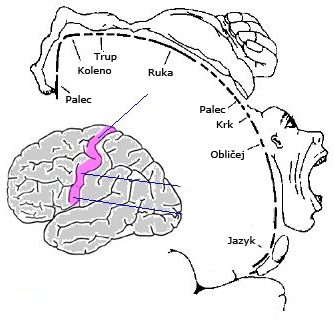
\includegraphics[scale=0.5]{casti/aplikace/sep/homunculus.jpg}
\caption{Homunkulus}
\end{figure}

Co se týče EEG signálu, hlavní složkou by měla být negativní vlna v dané oblasti, na kterou mohou navazovat další signály z okolních korových oblastí (z~primární i sekundární motorické oblasti a sekundární senzitivní oblasti), ty by ale měly mít nižší amplitudu. Vlna, kterou hledáme, by měla mít amplitudu přibližně 10~$\mu$V, její maximum se nachází asi po 19 ms po stimulačním impulsu (v závislosti na délce pacientovy paže se může čas maxima mírně lišit). \cite{68}

\begin{figure}[!h]
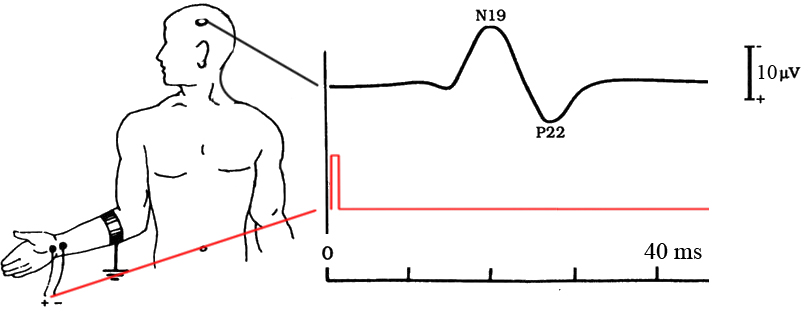
\includegraphics[scale=0.5]{casti/aplikace/sep/odezva.jpg}
\caption{Znázornění odezvy na stimul nervus medianus}
\end{figure}

